% EPT PWN Challenge #2 — assessment report
% Compile from 2_Final_Report/: pdflatex EPT_PWN2_Report.tex (run twice for TOC)
% Figures: filenames only; search path is ../1_Screenshots/

\documentclass[11pt]{article}
\usepackage[margin=1in]{geometry}
\usepackage{graphicx}
\graphicspath{{../1_Screenshots/}}
\usepackage[hidelinks]{hyperref}
\usepackage{booktabs}
\usepackage{caption}
\captionsetup{font=small,labelfont=bf}
\usepackage{array}
\usepackage{longtable}
\usepackage{fancyhdr}
\usepackage{lastpage}
\usepackage{xcolor}

\newcommand{\ScopeRange}{\texttt{10.20.160.10--200}}

\title{%
  Penetration Testing Report%
}
\author{%
  Student: Ariana Rocha (afrocha)\\
  Class: 95-483 Ethical Penetration Testing \\
  Assignment: PWN Challenge \#2 \\
}
\date{April 8, 2026}

\pagestyle{fancy}
\fancyhf{}
\lhead{PWN Challenge \#2}
\rhead{Ariana Rocha (afrocha)}
\cfoot{\thepage\ of \pageref{LastPage}}

\begin{document}

\maketitle
\vspace{0.75em}
\begin{center}
\fbox{\parbox{0.9\textwidth}{
\textbf{Scope (authorized)}: \ScopeRange \\[0.5em]
PWN Challenge \#2: identify and exploit in-scope hosts; document findings and evidence per the course rubric.
}}
\end{center}
\vspace{0.75em}
\begin{center}
\small\textit{Confidential — for course instructional use only.}
\end{center}
\vspace{0.75em}
\tableofcontents
\newpage

% --------------------------------------------------------------------------
\section{Executive Summary}
\label{sec:executive}

\noindent
This report summarizes a \textbf{time-limited penetration test} conducted against systems in an \textbf{authorized lab network segment}. The work focused on discovering live hosts, understanding exposed services, and validating whether an external attacker could gain operational control. Results are intended for \textbf{leadership and risk owners}: what was found, what it means for the organization, and what to do next.

\paragraph{Summary of findings.}
Testing produced \textbf{two complementary characterizations}. First, assessors \textbf{obtained interactive access} to one workstation via a \textbf{legacy, unsupported web-facing application}, establishing a \textbf{documented remote-code path} from the assessment network to that host. Second, a second workstation \textbf{presents a standard Windows SMB attack surface}; logged assessment showed \textbf{MS17-010--style checks reporting not vulnerable}, \textbf{limited unauthenticated enumeration}, and \textbf{documented credential testing with no successful authentication} in the captured runs. Post-examination on the compromised host included \textbf{structured enumeration} of user areas and disk paths consistent with the engagement objectives.

\paragraph{Business impact and associated risks.}
\textbf{Confirmed interactive access} on an endpoint demonstrates \textbf{confidentiality, integrity, and availability} risk for data and services that host can reach, \textbf{malware deployment} potential, and \textbf{lateral movement} feasibility. Separately, \textbf{exposed file-sharing} on an in-scope system---even where logged tests did not produce a shell---retains \textbf{credential-attack} and \textbf{unauthorized access} risk if accounts or permissions are weak. Together, these observations support \textbf{elevated operational and reputational risk} until remediated.

\paragraph{Recommendations.}
Prioritize \textbf{removal or replacement} of unsupported web software and \textbf{network segmentation} so administrative and user services are not broadly reachable. Harden \textbf{file-sharing}: least-privilege shares, strong passwords, lockout/monitoring, and \textbf{patch/lifecycle management} for legacy platforms. After remediation, \textbf{re-test} and document outcomes using the \textbf{course evidence standard}.

% --------------------------------------------------------------------------
\section{Detailed Findings}
\label{sec:findings}

Each finding below lists the elements required for grading: \textbf{name}, \textbf{description}, \textbf{severity}, \textbf{affected assets}, \textbf{mitigations}, and \textbf{evidence} (figures).

\subsection*{Summary table}
\begin{table}[htbp]
\centering
\caption{Finding summary (quick reference)}
\label{tab:findings-summary}
\begin{tabular}{@{}p{2cm}p{1.8cm}p{2.4cm}p{6.8cm}@{}}
\toprule
\textbf{ID} & \textbf{Severity} & \textbf{Asset(s)} & \textbf{Vulnerability (short)} \\
\midrule
F-001 & High & 10.20.160.112 (JUAN) & Legacy web service allowed remote session \\
F-002 & Low / Info & 10.20.160.63 (MATHIS) & SMB exposure; assessed exploitability and auth testing documented \\
\bottomrule
\end{tabular}
\end{table}

\subsection{Finding F-001: Legacy web service enabling remote session}
\label{finding:f001}

\begin{itemize}
  \item \textbf{Vulnerability name:} Legacy embedded web server (BadBlue-style stack) enabling remote access.
  \item \textbf{Description:} A workstation exposes an outdated HTTP service on a non-standard web port. Using the course Metasploit framework, assessors obtained an interactive Meterpreter session, demonstrating that an attacker could run code in the context of that machine.
  \item \textbf{Severity (criticality):} \textbf{High} --- remote code execution was demonstrated in the lab.
  \item \textbf{Affected hostnames / IPs:} Hostname \textbf{JUAN}; IP address \textbf{10.20.160.112}; service on \textbf{TCP 8080} (HTTP, BadBlue httpd 2.7 identified in scans).
  \item \textbf{Recommended mitigations:} Remove or replace unsupported software; restrict exposure to trusted networks; monitor for anomalous web-to-shell behavior; patch or retire vulnerable components.
  \item \textbf{Screenshot / evidence:} Figure~\ref{fig:finding-f001}.
\end{itemize}

\begin{figure}[htbp]
\centering
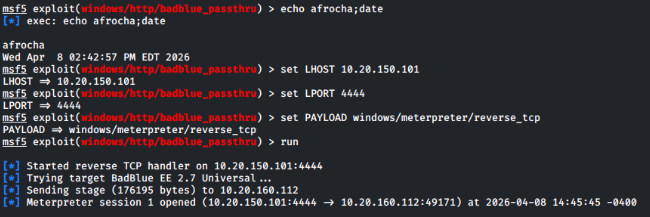
\includegraphics[width=0.92\textwidth]{14_badblue_exploit_success_meterpreter_session.png}
\caption{Evidence for Finding F-001: successful exploitation and Meterpreter session}
\label{fig:finding-f001}
\end{figure}

\subsection{Finding F-002: SMB exposure on MATHIS (assessed attack surface)}
\label{finding:f002}

\begin{itemize}
  \item \textbf{Vulnerability name:} Exposed Server Message Block (SMB) / NetBIOS services; exploitability assessed under the engagement methods used.
  \item \textbf{Description:} Host \textbf{MATHIS} runs Windows~7 Professional SP1 and listens for SMB on standard ports. Logged MS17-010--style checks \textbf{characterized the host as not appearing vulnerable} to that vector. Unauthenticated enumeration returned \textbf{limited share and identity detail}. Metasploit \texttt{smb\_login} with the documented wordlist produced \textbf{outcomes consistent with no matching credentials} in the captured run.
  \item \textbf{Severity (criticality):} \textbf{Low / Informational} for demonstrated remote takeover via the vectors exercised here; \textbf{medium concern} for ongoing attack surface if credentials or shares are weak.
  \item \textbf{Affected hostnames / IPs:} \textbf{MATHIS}; IP \textbf{10.20.160.63}; \textbf{TCP 139} and \textbf{TCP 445}.
  \item \textbf{Recommended mitigations:} Restrict SMB to required clients; enforce strong credentials and lockout policies; monitor authentication failures; migrate off end-of-life OS where feasible.
  \item \textbf{Screenshot / evidence:} Figure~\ref{fig:finding-f002}.
\end{itemize}

\begin{figure}[htbp]
\centering
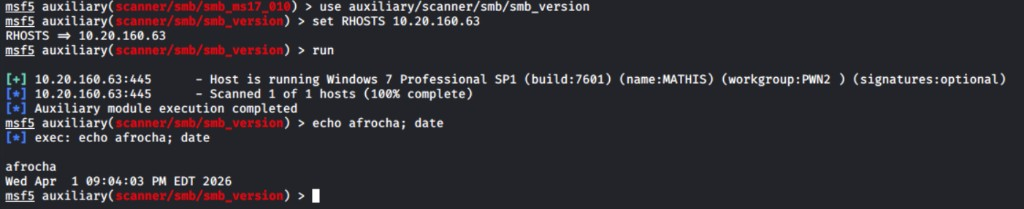
\includegraphics[width=0.92\textwidth]{08_smb_version_10.20.160.63_mathis_afrocha.png}
\caption{Evidence for Finding F-002: SMB and OS identification on MATHIS}
\label{fig:finding-f002}
\end{figure}

% --------------------------------------------------------------------------
\section{Technical Overview}
\label{sec:technical-overview}

This section is a \textbf{narrative walkthrough} of reconnaissance, exploitation, and post-exploitation. It is written so a \textbf{skilled technical reader} can follow the story line; \textbf{exact command strings} are collected in \textbf{Appendix~C} to avoid a play-by-play dump here (per rubric guidance). \textbf{Figures} support each major phase.

\subsection{Reconnaissance and enumeration}
Assessors discovered live systems in the authorized range using host discovery, then identified services with version detection. Two hosts remained the focus: one offered \textbf{SMB} (typical of Windows file sharing); the other offered \textbf{HTTP} on a high port consistent with an embedded web server. A follow-up port sweep checked common alternate services (including file transfer); \textbf{no additional high-value unauthenticated services} appeared on those standard ports in the logged run. Figures~\ref{fig:recon} and~\ref{fig:recon-sv} show stamped discovery and service identification.

\begin{figure}[htbp]
\centering
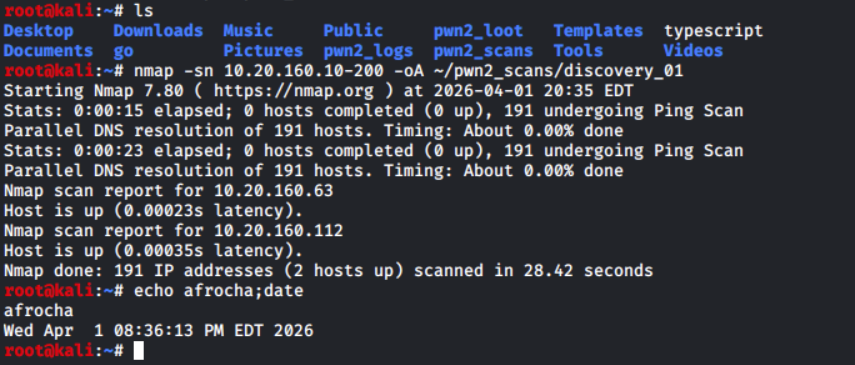
\includegraphics[width=0.92\textwidth]{01_discovery_nmap_sn_pwn2_scans_afrocha.png}
\caption{Discovery: ping sweep of authorized scope (identity stamp)}
\label{fig:recon}
\end{figure}

\begin{figure}[htbp]
\centering
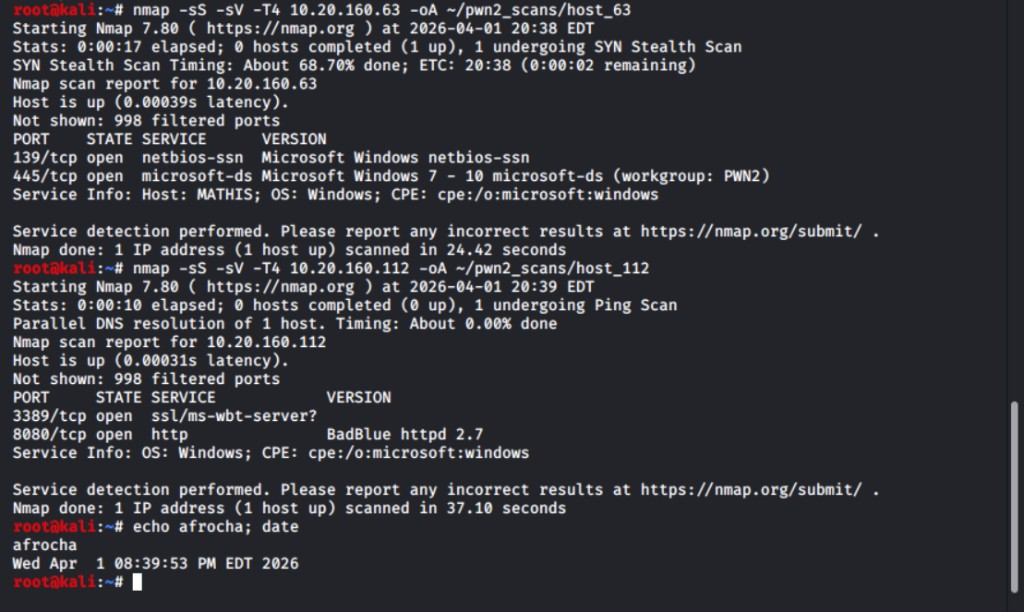
\includegraphics[width=0.92\textwidth]{02_hosts_63_112_nmap_sv_afrocha.png}
\caption{Service and version identification for both in-scope hosts}
\label{fig:recon-sv}
\end{figure}

\subsection{Initial access}
The team prioritized the \textbf{web-facing legacy service} on \textbf{10.20.160.112}. Using Metasploit, they selected a module matched to the product family, configured a reverse callback to the assessor-controlled system, and obtained a \textbf{Meterpreter session}. Figure~\ref{fig:initial-access} shows post-exploitation sanity checks from that session.

\begin{figure}[htbp]
\centering
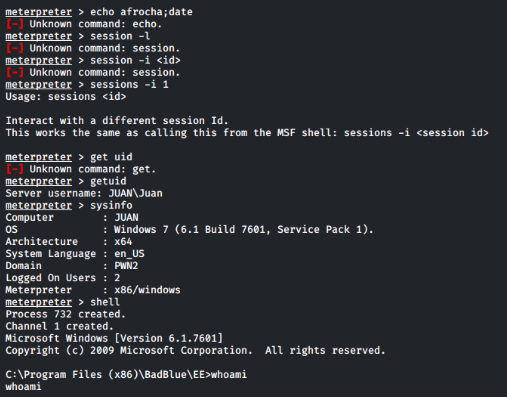
\includegraphics[width=0.92\textwidth]{15_meterpreter_interaction_sysinfo_shell_whoami.png}
\caption{Session validation after initial access (Meterpreter)}
\label{fig:initial-access}
\end{figure}

\subsection{Post-exploitation}
From the Windows shell, assessors performed \textbf{enumeration} of user profiles, desktops, and selected paths consistent with the engagement. In parallel, testing on the \textbf{SMB host} followed the \textbf{documented SMB methodology} (version and vulnerability characterization, authentication testing) summarized in Technical Details and the appendices.

% --------------------------------------------------------------------------
\section{Technical Details}
\label{sec:technical-details}

\subsection*{Summary table}
\begin{longtable}{@{}p{2.3cm}p{2cm}p{3.5cm}p{5.5cm}@{}}
\caption{Technical detail matrix (hostname/IP, ports, test outcome, exhibits)} \\
\toprule
\textbf{Hostname / IP} & \textbf{Open ports} & \textbf{Vulnerability / test result} & \textbf{Exhibits / notes} \\
\midrule
\endfirsthead
\multicolumn{4}{c}{\tablename\ \thetable\ -- \textit{continued}} \\
\toprule
\textbf{Hostname / IP} & \textbf{Open ports} & \textbf{Vulnerability / test result} & \textbf{Exhibits / notes} \\
\midrule
\endhead
\midrule
\multicolumn{4}{r}{\textit{Continued on next page}} \\
\endfoot
\bottomrule
\endlastfoot

JUAN / 10.20.160.112 &
8080 (HTTP BadBlue); RDP noted on broader scan &
Legacy HTTP service exploited; Meterpreter session established; post-ex enumeration per Technical Overview &
Session and exploitation evidence: Figure~\ref{fig:initial-access} \\

MATHIS / 10.20.160.63 &
139, 445 (SMB) &
SMB services characterized; logged MS17-style checks: not vulnerable; credential testing documented in work log &
SMB identification: Figure~\ref{fig:finding-f002} \\

\end{longtable}

\subsection{Host JUAN (10.20.160.112)}
\begin{itemize}
  \item \textbf{Hostname and IP address:} JUAN; \textbf{10.20.160.112}
  \item \textbf{Open ports:} \textbf{TCP 8080} (primary); remote desktop observed in broader recon where applicable.
  \item \textbf{Vulnerability description:} Legacy BadBlue-class HTTP service allowing remote code execution via Metasploit \texttt{badblue\_passthru} and \texttt{windows/meterpreter/reverse\_tcp} (see Technical Overview).
\end{itemize}

\subsection{Host MATHIS (10.20.160.63)}
\begin{itemize}
  \item \textbf{Hostname and IP address:} MATHIS; \textbf{10.20.160.63}
  \item \textbf{Open ports:} \textbf{TCP 139}, \textbf{TCP 445}
  \item \textbf{Vulnerability description:} SMB attack surface; logged testing produced \textbf{MS17-negative characterization}; authentication testing is summarized in the course work log; remote shell not within the access level established for this host in the captured runs.
\end{itemize}

% --------------------------------------------------------------------------
\appendix
\section{Appendix A: Scope and rules of engagement}
\label{app:roe}

\begin{itemize}
  \item Authorized scope: \ScopeRange.
  \item Testing limited to course lab systems and engagement rules.
  \item Identity stamps: \texttt{echo afrocha; date} on Kali; Windows \texttt{echo afrocha \%date\% \%time\%} in shells where applicable.
\end{itemize}

\section{Appendix B: Documentation and prior feedback}
\label{app:doc-standards}

\begin{itemize}
  \item \textbf{Reproducibility:} Findings are supported by stamped screenshots and command references so a reviewer can relate evidence to conclusions.
  \item \textbf{Scoped outcomes:} Where a host is characterized without shell access (e.g.\ MATHIS SMB), the report documents \textbf{methods, tools, and observed results} so conclusions remain traceable, consistent with prior course feedback.
\end{itemize}

\section{Appendix C: Tooling}
\label{app:tools}

\begin{itemize}
  \item Kali Linux (course VM); Metasploit Framework
  \item Nmap 7.x
  \item Evidence repository: \texttt{1\_Screenshots/}; work log \texttt{3\_Work/README.md}
\end{itemize}

\section{Appendix D: Raw command reference}
\label{app:commands}

\begin{itemize}
  \item Discovery: \texttt{nmap -sn 10.20.160.10-200}
  \item Service scan: \texttt{nmap -sS -sV -T4} per host
  \item Focused ports: \texttt{nmap -p 21,80,8080,443,139,445 --open -sV 10.20.160.63 10.20.160.112}
  \item SMB scripts (optional): \texttt{nmap --script smb-enum-shares,smb-enum-users -p139,445 10.20.160.63}
  \item Exploit: \texttt{exploit/windows/http/badblue\_passthru}, \texttt{RPORT 8080}, payload \texttt{windows/meterpreter/reverse\_tcp}
  \item MATHIS: \texttt{auxiliary/scanner/smb/smb\_login} on port 445 with \texttt{USER\_FILE} / \texttt{PASS\_FILE}
  \item Proof hunt (Windows): recursive file search and \texttt{findstr} filtering (see course repo \texttt{README.md})
\end{itemize}

\section{Appendix E: Limitations and submission notes}
\label{app:limitations}

\begin{itemize}
  \item \textbf{Evidence package:} Primary exhibits in this PDF are \textbf{reconnaissance}, \textbf{successful exploitation (JUAN)}, and \textbf{SMB characterization (MATHIS)}; supplementary command detail appears in the repository work log where needed.
  \item \textbf{MATHIS:} Findings describe \textbf{SMB exposure and assessed exploitability} under the logged test plan; treat as \textbf{attack-surface intelligence} alongside JUAN results.
  \item \textbf{Scope drift:} Re-run discovery if the lab adds additional live hosts.
\end{itemize}

\end{document}
